\documentclass[12pt, t]{beamer}

%------------------------------------------------------------------------------
% doc
%------------------------------------------------------------------------------
%https://fr.wikipedia.org/wiki/Noyau_de_syst%C3%A8me_d%27exploitation
%http://infomaroon.blogspot.fr/2008/04/diffrents-types-de-noyaux.html
%http://etud.insa-toulouse.fr/~projet_tut_OS/w/Noyaux_monolithiques

%------------------------------------------------------------------------------
% configuration
%------------------------------------------------------------------------------
\RequirePackage{etex}
\usepackage{currfile-abspath}
\usepackage{../../themes/dbt}
\usepackage{catchfilebetweentags}

\setbeameroption{hide notes}
\setbeamertemplate{caption}{\raggedright\insertcaption\par}

\graphicspath{{images/}}
\getmainfile
\getabspath{\themainfile}
\let\mainabsdir\theabsdir
\let\mainabspath\theabspath

\newcommand{\insertcode}[2]{\lstinputlisting[label=samplecode, basicstyle=#1]{\mainabsdir/code/#2}}
\newcommand{\bi}{\begin{itemize}}
\newcommand{\ei}{\end{itemize}}
\newcommand{\ig}{\includegraphics}
\newcommand{\myhref}[1]{\href{#1}{\tt \scriptsize #1}}
\newcommand{\incnote}[1]{\note{\ExecuteMetaData[notes.tex]{#1}}}
\newcommand{\src}[2]{\vspace{-10pt}\caption{\href{#1}{\centering \tt \tiny [#2]}}}


%------------------------------------------------------------------------------
% title
%------------------------------------------------------------------------------
%------------------------------------------------------------------------------
% title
%------------------------------------------------------------------------------
% slide
\title{Systèmes d'exploitation pour l'embarqué}
\subtitle{UV 5.2 - Exécution et Concurrence}

\author{\href{}{Paul Blottière}}
\institute{
    \href{http://www.ensta-bretagne.fr/}{ENSTA Bretagne} \\[2pt]
    \href{}{\tt \scriptsize 2018 / 2019}
}
\date{
    \href{https://github.com/pblottiere}{\tt \scriptsize https://github.com/pblottiere} \\[2pt]
    %\href{blottiere.paul@gmail.com}{\tt \scriptsize blottiere.paul@gmail.com}
}

% info
\begin{document}

{
\setbeamertemplate{footline}{} % no page number here
\frame{
    \titlepage
} }

%------------------------------------------------------------------------------
% amélioration continue
%------------------------------------------------------------------------------
\begin{frame}{Amélioration continue}
    \subt{Contributions}
    \vspace{12pt}

    \begin{center}
    
\includegraphics[scale=0.7]{github.png}
    \end{center}

    \bi
    \itemsep12pt
    \item Dépôt du cours : \href{https://github.com/pblottiere/embsys}{\tt \scriptsize https://github.com/pblottiere/embsys}
    \item Souhaits d'amélioration, erreurs, idées de TP, ... : ouverture d'Issues
    \item Apports de corrections : Pull Request
    \ei
\end{frame}




%<**lecture_content>
%------------------------------------------------------------------------------
% lecture
%------------------------------------------------------------------------------
\begin{frame}[plain,c]
    \centering
    \huge\textcolor{title}{Kernel Linux et modules - version 2.6.x}
\end{frame}

%------------------------------------------------------------------------------
% plan
%------------------------------------------------------------------------------
\begin{frame}{Plan}
    \subt{}
    \vspace{10pt}

    \begin{enumerate}
        \itemsep12pt
        \item Noyau : généralités
        \item user-space et kernel-space
        \item Architectures noyaux
        \item Phases de boot
        \item Périphérique bloc ou caractère
        \item Administrer les modules sous Linux
        \item Développement de module kernel
    \end{enumerate}

    \note {
    }
\end{frame}

%------------------------------------------------------------------------------
% gen1
%------------------------------------------------------------------------------
\begin{frame}{Noyau : généralités (1)}
    \subt{Les fonctions d'un kernel}

    \vspace{5pt}
    Le noyau d'un système d'exploitation :
    \vspace{3pt}
    \bi
    \itemsep4pt
    \item gère la partie matérielle (mémoire, processeurs, périphériques, ...)
    \item offre la gestion des ressources matérielles à travers des appels
          système
    \item gère les tâches à exéctuer (ordonnancement)
    \ei

    \onslide<2->
    {
        \begin{figure}
            \centering
            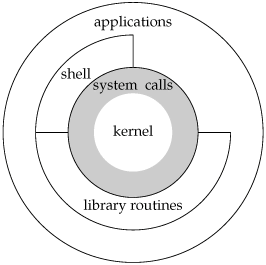
\includegraphics[scale=0.5]{kernel.png}
            \src{https://dimaslviv.wordpress.com/author/dimaslviv/}{Couches d'un OS}
        \end{figure}
    }

\end{frame}

%------------------------------------------------------------------------------
% gen2
%------------------------------------------------------------------------------
\begin{frame}{Noyau : généralités (2)}
    \subt{Les enjeux}

    \vspace{15pt}
    La programmation kernel nécessite une attention particulière sur :
    \vspace{8pt}
    \bi
    \itemsep12pt
    \item les problèmes de performance
    \item les failles de sécurité
    \item le système de fichiers (corruption)
    \item la gestion mémoire
    \ei

\end{frame}

%------------------------------------------------------------------------------
% uk1
%------------------------------------------------------------------------------
\begin{frame}{user-space et kernel-space (1)}
    \subt{Ring}

    \vspace{8pt}
    L'architecture même d'un processeur impose des niveaux de privilèges pour
    accéder et sécuriser l'accès aux instructions, à l'espace d'adressage
    ou aux entrées-sorties.

    \onslide<2->
    {
        \vspace{8pt}
        Ces niveaux sont appelés {\textbf{Anneaux de protection} ou \textbf{Rings}}.

        \begin{figure}
            \centering
            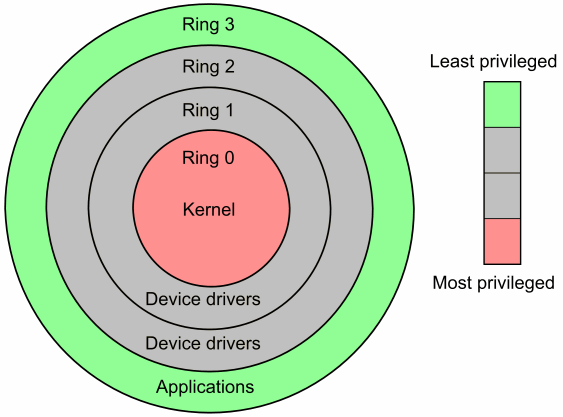
\includegraphics[scale=0.25]{ring.png}
        \end{figure}
    }

\end{frame}

%------------------------------------------------------------------------------
% uk2
%------------------------------------------------------------------------------
\begin{frame}{user-space et kernel-space (2)}
    \subt{Ring}

    \vspace{10pt}
    Dans un processeur x86, la notion d'anneau est représentée via le champ
    {\textbf{Input/Output Privilege Level}} du registre EFLAG :

    \vspace{10pt}
    \begin{figure}
        \centering
        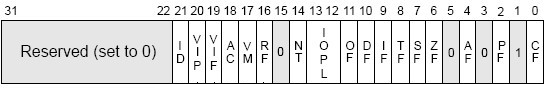
\includegraphics[scale=0.7]{eflag.png}
    \end{figure}

    \onslide<2->{
        \vspace{8pt}
        => le champ IOPL ne peut être modifié qu'avec le niveau de privilège le
        plus élevé!
    }

\end{frame}

%------------------------------------------------------------------------------
% uk3
%------------------------------------------------------------------------------
\begin{frame}{user-space et kernel-space (3)}
    \subt{Besoin d'espace}

    \vspace{20pt}
    Un OS moderne possède deux espaces mémoire distincts :
    \vspace{8pt}
    \bi
    \itemsep12pt
    \item Espace utilisateur : programmes qui discutent avec le matériel à
          travers le kernel via les appels système. Chaque processus exécuté
          dans l'espace utilisateur possède sa propre plage de mémoire virtuelle.
    \onslide<2->{
        \item Espace kernel : réservé pour le kernel et ses drivers. Possède le
              niveau de privilège le plus élevé.
        \ei
    }

\end{frame}

%------------------------------------------------------------------------------
% arch2
%------------------------------------------------------------------------------
\begin{frame}{Architectures noyaux (2)}
    \subt{Noyaux monolithiques non modulaires}

    \vspace{10pt}
    Dans un noyau monolithique pur (comprendre non modulaire), tous les pilotes
    de périphériques sont compilés avec le noyau pour former un seul binaire.

    \onslide<2->
    {
        \vspace{5pt}
        \begin{figure}
            \centering
            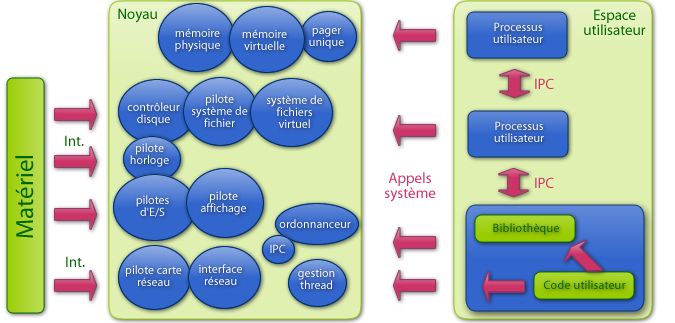
\includegraphics[scale=0.44]{mono.png}
            \src{https://fr.wikipedia.org/wiki/Noyau\_de\_syst\%C3\%A8me\_d\%27exploitation}{Kernel monolithique}
        \end{figure}
    }

\end{frame}

%------------------------------------------------------------------------------
% arch3
%------------------------------------------------------------------------------
\begin{frame}{Architectures noyaux (3)}
    \subt{Noyaux monolithiques non modulaires}

    \vspace{10pt}
    Les avantages :
    \vspace{5pt}
    \bi
    \itemsep8pt
    \item architecture simple
    \item vitesse d'exécution
    \ei

    \onslide<2->
    {
        \vspace{10pt}
        Les inconvénients :
        \vspace{5pt}
        \bi
        \itemsep8pt
        \item empreinte mémoire dépendante du nombre de drivers
        \item difficile à maintenir
        \item une erreur dans un driver met en danger tout le système (kernel
              space)
        \ei
    }

\end{frame}

%------------------------------------------------------------------------------
% arch4
%------------------------------------------------------------------------------
\begin{frame}{Architectures noyaux (4)}
    \subt{Noyaux monolithiques modulaires}

    \vspace{15pt}
    Dans un noyau monolithique modulaire, on choisit au moment de la compilation
    du kernel si un driver doit être inclus dans le "binaire kernel" ou
    bien compilé en tant que {\textbf{module}}.

    \onslide<2->
    {
        \vspace{15pt}
        Un module peut être chargé à la volée pour rajouter une fonctionnalité
        (comme gérer un nouveau type de matériel).
    }

    \onslide<3->
    {
        \vspace{15pt}
        Mais, une erreur dans un module, même chargé à chaud, met toujours la
        stabilité du système en péril.
    }

\end{frame}

%------------------------------------------------------------------------------
% arch5
%------------------------------------------------------------------------------
\defverbatim{\lstconf}{
    \begin{lstlisting}
    > uname -r
    4.1.0-2-686-pae
    > tail /boot/config-4.1.0-2-686-pae
    CONFIG_AVERAGE=y
    CONFIG_CORDIC=m
    # CONFIG_DDR is not set
    CONFIG_OID_REGISTRY=m
    CONFIG_UCS2_STRING=y
    CONFIG_FONT_SUPPORT=y
    # CONFIG_FONTS is not set
    \end{lstlisting}
}

\begin{frame}{Architectures noyaux (5)}
    \subt{Noyaux monolithiques modulaires}

    \vspace{10pt}
    Depuis la version 1.2 de Linux, l'architecture est modulaire.

    \onslide<2->
    {
        \vspace{10pt}
        Les modules kernel sont indiqués via un {\textbf{m}} dans la configuration
        du noyau :

        \vspace{8pt}
        \lstconf
    }

\end{frame}

%------------------------------------------------------------------------------
% arch6
%------------------------------------------------------------------------------
\begin{frame}{Architectures noyaux (6)}
    \subt{Micro-noyaux}

    \vspace{8pt}
    Un micro-noyau est beaucoup plus léger/petit qu'un noyau monolithique :
    6 millions de LOC pour Linux contre moins de 50 000 LOC pour un micro-noyau.

    \onslide<2->
    {
        \vspace{8pt}
        La plupart des services d'un noyau monolithique sont ici exécutés dans
        l'espace utilisateur via des serveurs de fonctionnalités, réduisant ainsi le
        volume du kernel.

        \begin{figure}
            \centering
            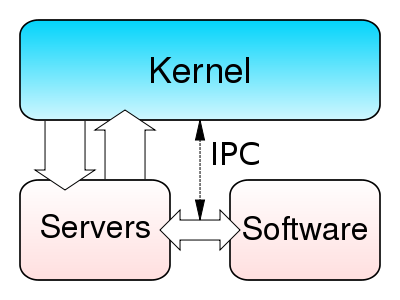
\includegraphics[scale=0.32]{micro.png}
            \src{http://malhar2010.blogspot.fr/2010/11/types-of-kernel.html}{Micro kernel}
        \end{figure}
    }

\end{frame}

%------------------------------------------------------------------------------
% arch7
%------------------------------------------------------------------------------
\begin{frame}{Architectures noyaux (7)}
    \subt{Micro-noyaux}

    \vspace{15pt}
    Les avantages :
    \vspace{5pt}
    \bi
    \itemsep8pt
    \item kernel facile à maintenir de par le faible volume de code
    \item une erreur dans un driver ne remet pas en cause la stabilité du
          système (exécuté dans l'espace utilisateur : mode protégé)
    \ei

    \onslide<2->
    {
        \vspace{15pt}
        Les inconvénients :
        \vspace{5pt}
        \bi
        \itemsep8pt
        \item lent car beaucoup d'appels système pour assurer la communication
              entre serveurs et kernel.
          \item communication entre services très lourde (IPC).
        \ei
    }

\end{frame}

%------------------------------------------------------------------------------
% arch8
%------------------------------------------------------------------------------
\begin{frame}{Architectures noyaux (8)}
    \subt{Noyaux temps réel}

    \vspace{10pt}
    L'architecture classique est un noyau hybride combinant un noyau monolithique
    généraliste avec un micro-noyau spécialisé temps-réel.

    \onslide<2->
    {
        \vspace{10pt}
        Le noyau généraliste est considéré par le micro-noyau comme un service.

        \vspace{10pt}
        \begin{figure}
            \centering
            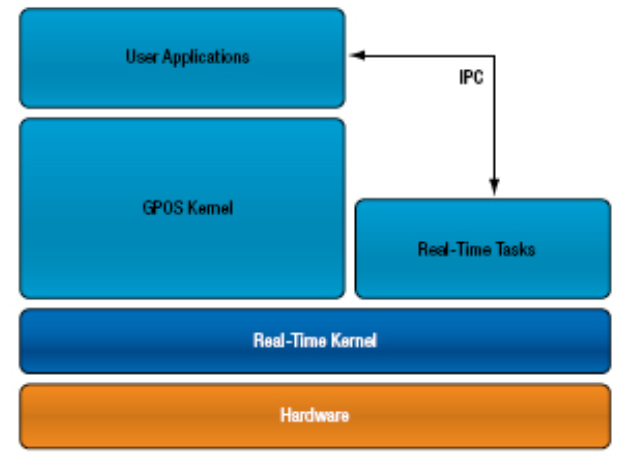
\includegraphics[scale=0.3]{rt.png}
            \src{http://www.rtcmagazine.com/articles/view/101091}{Noyau temps réel}
        \end{figure}
    }

\end{frame}

%------------------------------------------------------------------------------
% boot1
%------------------------------------------------------------------------------
\begin{frame}{Phases de boot (1)}
    \subt{BIOS, UEFI et bootloader}

    \vspace{10pt}
    {\textbf{BIOS (Basic Input/Output System)}} : firmware présent sur la
    mémoire flash de la carte mère. Il lit le MBR (Master Boot Record : premier
    secteur de 512 o d'un disque dur) pour déterminer la position du bootloader
    et le lancer.

    \vspace{8pt}
    => taille des partitions limitée à 2.2 To

    \onslide<2->
    {
        \vspace{10pt}
        {\textbf{UEFI (Unified Extensible Firmware Interface)}} : lit la GPT du
        disque pour déterminer la position du bootloader et le lancer.

        \vspace{8pt}
        => taille des partitions limitée à 9.4 Zo %(10\^21)
    }

    \onslide<3->
    {
        \vspace{10pt}
        {\textbf{Bootloader (chargeur d'amorçage)}} : permet à l'utilisateur de
        choisir le système d'exploitation à lancer (multi-boot). Il est
        notamment chargé d'exécuter le kernel.
    }

\end{frame}

%------------------------------------------------------------------------------
% boot2
%------------------------------------------------------------------------------
\begin{frame}{Phases de boot (2)}
    \subt{filesystem}

    \vspace{15pt}
    Le bootloader, en plus de lancer le kernel, charge en mémoire une image
    compressée du système de fichiers (initrd, initramfs, ...).

    \onslide<2->
    {
        \vspace{15pt}
        Le kernel décompresse ensuite l'image et monte le système de fichiers. On
        a alors le RFS (Root FileSystem).

        \begin{figure}
            \centering
            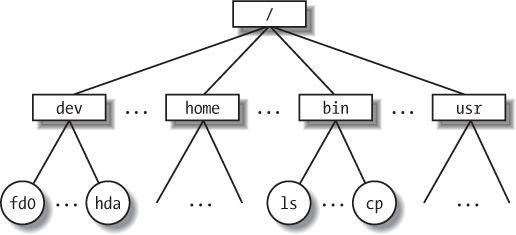
\includegraphics[scale=0.4]{rfs.png}
        \end{figure}
    }

\end{frame}

%------------------------------------------------------------------------------
% boot3
%------------------------------------------------------------------------------
\defverbatim{\lstboot}{
    \begin{lstlisting}
> cat /proc/cmdline
BOOT_IMAGE=/boot/vmlinuz-4.1.0-2-686-pae \
    root=UUID=4dbf9632-e453-43e9-af6f-4d8bbaa4186f \
    ro quiet
    \end{lstlisting}
}

\begin{frame}{Phases de boot (3)}
    \subt{init}

    \vspace{15pt}
    Par défaut, le kernel lance la phase d'initialisation en utilisant le binaire
    {\textbf{/sbin/init}} du RFS. On peut indiquer un autre programme
    d'initialisation grâce à l'option {\textbf{init=}}.

    \vspace{10pt}
    \lstboot

    \onslide<2->
    {
        \vspace{10pt}
        Le processus {\textbf{init}} est le père de tous les processus et possède
        un PID=1!
    }

    \onslide<3->
    {
        \vspace{10pt}
        Le binaire d'initialisation consulte le fichier {\textbf{inittab}} pour
        connaître l'ordre dans lequel il doit démarrer les processus du système.
    }

\end{frame}

%------------------------------------------------------------------------------
% boot4
%------------------------------------------------------------------------------
\begin{frame}{Phases de boot (4)}
    \subt{run-levels}

    \vspace{15pt}
    Le niveau d'exécution, ou runlevel, contrôle le choix des processus
    démarrés automatiquement par le système :

    \vspace{8pt}
    \bi
    \itemsep8pt
    \item 0 : arrêt du système
    \item 1 ou S : mode maintenance
    \item 2, 3, 4 ou 5 : mode multi-utilisateurs
    \item 6 : redémarrage du système
    \ei

    \onslide<2->
    {
        \vspace{8pt}
        Un RC (Run Command) est un processus qui se lance au démarrage du système
        à un runlevel particulier et se termine à un autre runlevel.
    }

\end{frame}

%------------------------------------------------------------------------------
% boot5
%------------------------------------------------------------------------------
\defverbatim{\lstrc}{
    \begin{lstlisting}
> head /etc/init.d/networking
#!/bin/sh -e
### BEGIN INIT INFO
# Provides:          networking ifupdown
# Required-Start:    mountkernfs local_fs random
# Required-Stop:     local_fs
# Default-Start:     S
# Default-Stop:      0 6
# Short-Description: Raise network interfaces.
# Description:       Prepare /run/network ...
### END INIT INFO
    \end{lstlisting}
}

\begin{frame}{Phases de boot (5)}
    \subt{run-levels}

    \vspace{30pt}
    Run-levels du service réseau :
    \vspace{10pt}
    \lstrc

\end{frame}

%------------------------------------------------------------------------------
% dev1
%------------------------------------------------------------------------------
\begin{frame}{Périphérique bloc ou caractère (1)}
    \subt{/dev}

    \vspace{20pt}
    Le répertoire {\textbf{/dev}} du RFS offre un moyen de communiquer
    directement avec le materiel.

    \onslide<2->
    {
        \vspace{20pt}
        Ce répertoire peut être soit peuplé de manière fixe, soit peuplé au moment
        du boot par scan du materiel présent (par l'utilitaire {\textbf{udev}}).
    }

    \onslide<3->
    {
        \vspace{20pt}
        Dans le cas d'un fichier spécial de périphérique matériel, il existe deux
        types : bloc ou caractère.
    }

\end{frame}

%------------------------------------------------------------------------------
% dev2
%------------------------------------------------------------------------------
\defverbatim{\lstnod}{
    \begin{lstlisting}
# mknod rights name type major-number minor-number
> mknod -m 622 RFS_PATH/dev/console c 5 1
> mknod -m 666 RFS_PATH/dev/null c 1 3
> mknod -m 444 RFS_PATH/dev/urandom c 1 9
    \end{lstlisting}
}

\begin{frame}{Périphérique bloc ou caractère (2)}
    \subt{mknod}

    \vspace{10pt}
    L'utilitaire {\textbf{mknod}} peut être utilisé pour créer des noeuds au
    sein du système de fichiers :

    \vspace{10pt}
    \lstnod

    \onslide<2->
    {
        Signification des numéros :
        \bi
        \item majeur : permet au kernel de déterminer quel pilote utiliser lors
              d'une écriture/lecture/ouverture sur le noeud
        \item mineur : réservé au pilote pour différencier des sous catégories
              d'un même type de matériel.
        \ei
    }

\end{frame}

%------------------------------------------------------------------------------
% dev3
%------------------------------------------------------------------------------
\defverbatim{\lstbloc}{
    \begin{lstlisting}
> ls -l /dev/sda[1-3]
brw-rw---- 1 root disk 8, 1 déc.   3 21:50 /dev/sda1
brw-rw---- 1 root disk 8, 2 déc.   3 21:50 /dev/sda2
brw-rw---- 1 root disk 8, 3 déc.   3 21:50 /dev/sda3
    \end{lstlisting}
}

\begin{frame}{Périphérique bloc ou caractère (3)}
    \subt{block device}

    \vspace{20pt}
    L'accès à une ressource matérielle à travers un fichier spécial de type bloc
    est bufferisé. Les commandes demandées peuvent même être réorganisées pour
    optimiser les accès en écriture/lecture.

    \onslide<2->
    {
        \vspace{20pt}
        Les périphériques de stockage sont donc de type bloc :
        \vspace{5pt}
        \lstbloc
    }

\end{frame}

%------------------------------------------------------------------------------
% dev4
%------------------------------------------------------------------------------
\defverbatim{\lstchar}{
    \begin{lstlisting}
> ls -l /dev/ttyS[0-3]
crw-rw---- 1 root dial 4, 64 déc. 3 21:50 /dev/ttyS0
crw-rw---- 1 root dial 4, 65 déc. 3 21:50 /dev/ttyS1
crw-rw---- 1 root dial 4, 66 déc. 3 21:50 /dev/ttyS2
crw-rw---- 1 root dial 4, 67 déc. 3 21:50 /dev/ttyS3
    \end{lstlisting}
}

\begin{frame}{Périphérique bloc ou caractère (4)}
    \subt{character device}

    \vspace{20pt}
    L'accès à une ressource matérielle via un fichier de type caractère est
    direct et non bufferisé. La plupart des périphériques sont de type
    caractère.

    \onslide<2->
    {
        \vspace{20pt}
        \lstchar
    }

\end{frame}

%------------------------------------------------------------------------------
% admin1
%------------------------------------------------------------------------------
\begin{frame}{Administrer les modules sous Linux (1)}
    \subt{Où sont-ils?}

    \vspace{3pt}
    Sous Linux, un module kernel étend sans reboot les fonctionnalités du noyau
    et est représenté par des fichiers ayant l'extension {\textbf{.ko}} (comme
    Kernel Object).

    \begin{figure}
        \centering
        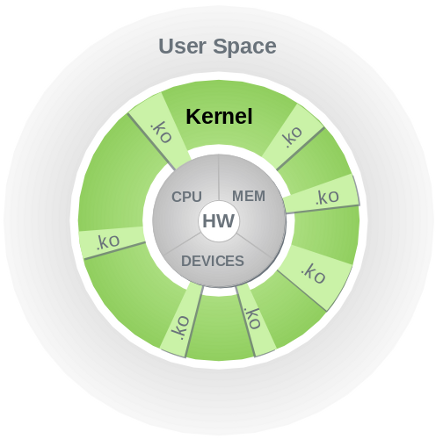
\includegraphics[scale=0.6]{modules.png}
        \src{https://drivers.suse.com/doc/SolidDriver/Kernel_Modules.html}{Modules}
    \end{figure}

    \onslide<2->
    {
        \vspace{-14pt}
        Les modules sont présents dans le répertoire
        {\textit{/lib/modules/version}}.
    }

\end{frame}

%------------------------------------------------------------------------------
% admin2
%------------------------------------------------------------------------------
\defverbatim{\lstkmod}{
    \begin{lstlisting}
load_module() {
  local module args
  module="$1"
  args="$2"

  if [ "$VERBOSE" != no ]; then
    log_action_msg "Loading kernel module $module"
    modprobe $module $args || true
  else
    modprobe $module $args > /dev/null 2>&1 || true
  fi
}
    \end{lstlisting}
}

\begin{frame}{Administrer les modules sous Linux (2)}
    \subt{Phases de chargement}

    \vspace{15pt}
    Lorsque le kernel a besoin d'une fonctionnalité qu'il ne trouve pas dans son
    espace, le démon kernel {\textbf{kmod}} lance l'utilitaire {\textbf{modprobe}}
    pour charger le module :

    \vspace{10pt}
    \lstkmod

\end{frame}

%------------------------------------------------------------------------------
% admin3
%------------------------------------------------------------------------------
\defverbatim{\lstdep}{
    \begin{lstlisting}
> insmod /lib/modules/ver/kernel/fs/fat/fat.ko
> insmod /lib/modules/ver/kernel/fs/msdos/msdos.ko
    \end{lstlisting}
}

\defverbatim{\lstdepbis}{
    \begin{lstlisting}
> modprobe msdos
    \end{lstlisting}
}

\begin{frame}{Administrer les modules sous Linux (3)}
    \subt{Phases de chargement}

    \vspace{8pt}
    Des modules peuvent avoir des dépendances vers d'autres modules. L'utilitaire
    {\textbf{modprobe}} va chercher ces dépendances dans le fichier
    {\textit{/lib/modules/version/modules.dep}}.

    \onslide<2->
    {
        \vspace{8pt}
        Suite à cela, la commande {\textbf{insmod}} est utilisée pour charger les
        modules prérequis puis le module en question.
    }

    \onslide<3->
    {
        \vspace{8pt}
        Par exemple :
        \vspace{4pt}
        \lstdep
        équivaut à :
        \vspace{4pt}
        \lstdepbis
    }

\end{frame}

%------------------------------------------------------------------------------
% admin5
%------------------------------------------------------------------------------
\begin{frame}{Administrer les modules sous Linux (5)}
    \subt{Déchargement}

    \vspace{20pt}
    Un module ne peut pas être déchargé si il est actuellement utilisé ou
    nécessaire pour d'autres modules chargés.

    \onslide<2->
    {
        \vspace{20pt} On peut voir le nombre de processus utilisant un module via
        la commande {\textbf{lsmod}} ou bien en étudiant le troisième champ du
        fichier virtuel {\textbf{/proc/modules}}.
    }

    \onslide<3->
    {
        \vspace{20pt}
        Le déchargement d'un module se fait via la commande {\textbf{rmmod}}.
    }

\end{frame}

%------------------------------------------------------------------------------
% mod1
%------------------------------------------------------------------------------
\begin{frame}{Développement de module kernel (1)}
    \subt{La base}

    \vspace{10pt}
    Deux fonctions sont nécessaires dans un module kernel :
    \bi
    \itemsep8pt
    \item une fonction d'initialisation appelée au moment de l'appel de
        {\textbf{insmod}} et enregistrée via {\textbf{module\_init}}.
    \item une fonction de nettoyage appelée juste avant le déchargement du
          module et enregistrée via {\textbf{module\_exit}}.
    \ei

    \onslide<2->
    {
        \vspace{10pt}
        Un module peut être documenté via des macros comme
        {\textbf{MODULE\_AUTHOR}} ou {\textbf{MODULE\_DESCRIPTION}}.

        \vspace{10pt}
        => ces informations sont ensuite consultables grâce à la commande
        {\textbf{modinfo}}.
    }

\end{frame}

%------------------------------------------------------------------------------
% mod2
%------------------------------------------------------------------------------
\defverbatim{\lstsyms}{
    \begin{lstlisting}
> head -5 /proc/kallsyms
c1000358 T _stext
c1001000 T hypercall_page
c1001000 t xen_hypercall_set_trap_table
c1001020 t xen_hypercall_mmu_update
c1001040 t xen_hypercall_set_gdt
    \end{lstlisting}
}

\begin{frame}{Développement de module kernel (2)}
    \subt{Les appels système}

    \vspace{12pt}
    Un module étant exécuté dans l'espace kernel, il n'a pas accès aux
    librairies fournies par le système d'exploitation comme la glibc.

    \onslide<2->
    {
        \vspace{12pt}
        Seules les fonctions fournies par le kernel lui même sont accessibles. Elles
        sont définies dans le fichier virtuel /proc/kallsyms :

        \vspace{12pt}
        \lstsyms
    }

\end{frame}

%------------------------------------------------------------------------------
% mod3
%------------------------------------------------------------------------------
\begin{frame}{Développement de module kernel (3)}
    \subt{printk : mécanisme de log kernel avec niveaux de priorité}

    \lstinputlisting[label=samplecode, basicstyle=\scriptsize]{code/module_printk.c}

\end{frame}

%------------------------------------------------------------------------------
% mod4
%------------------------------------------------------------------------------
\defverbatim{\lstload}{
    \begin{lstlisting}
> insmod custommodule.ko param1=3
    \end{lstlisting}
}

\defverbatim{\lstparam}{
    \begin{lstlisting}
static type varname = initial_value;
module_param(varname, type, rights);
MODULE_PARAM_DESC(varname, "VARNAME DOCUMENTATION")
    \end{lstlisting}
}

\begin{frame}{Développement de module kernel (4)}
    \subt{Paramètres}

    \vspace{15pt}
    Un module peut prendre des paramètres au moment de son chargement :

    \vspace{6pt}
    \lstload

    \onslide<2->
    {
        \vspace{15pt}
        Pour cela, les paramètres doivent être enregistrés via la fonction
        {\textbf{module\_param}} et documentés via
        {\textbf{MODULE\_PARM\_DESC}} :

        \vspace{6pt}
        \lstparam
    }

\end{frame}

%------------------------------------------------------------------------------
% mod5
%------------------------------------------------------------------------------
\begin{frame}{Développement de module kernel (5)}
    \subt{Configuration et /proc}

    \vspace{20pt}
    Un module kernel peut lire et écrire des fichiers dans le répertoire
    {\textbf{/proc}}. Un utilisateur peut alors configurer le comportement
    du module via l'édition de ces fichiers.

    \vspace{20pt}
    Pour cela, les fonctions {\textbf{create\_proc\_entry}}, {\textbf{copy\_to\_user}}
    et {\textbf{copy\_from\_user}} sont utilisées.

    \onslide<2->
    {
        \vspace{20pt}
        Remarque : dans le monde kernel, le référentiel est l'utilisateur. Ainsi,
        une fonction de lecture définie dans le module va écrire des données alors
        qu'une fonction d'écriture va en lire.
    }

\end{frame}

%------------------------------------------------------------------------------
% mod6
%------------------------------------------------------------------------------
\defverbatim{\lstfops}{
    \begin{lstlisting}
struct file_operations fops = {
    .read = custom_device_read,
    .open = custom_device_open
};
    \end{lstlisting}
}

\begin{frame}{Développement de module kernel (6)}
    \subt{Character device}

    \vspace{15pt}
    Plusieurs opérations sont possibles sur le matériel : écriture, lecture,
    configuration, flush, ... Ces actions sont représentées par des pointeurs
    de fonctions dans la structure {\textbf{file\_operations}}.

    \onslide<2->
    {
        \vspace{15pt}
        Par défaut, les actions pointent vers NULL. Si le développeur du module
        veut customiser l'action d'ouverture et de lecture du device :
        \vspace{8pt}
        \lstfops
    }

\end{frame}

%------------------------------------------------------------------------------
% mod7
%------------------------------------------------------------------------------
\begin{frame}{Développement de module kernel (7)}
    \subt{Les états}

    \vspace{15pt}
    Un module peut gérer l'état des tâches qui communiquent avec lui et même
    les ajouter dans des WaitQ que le scheduler réveillera au moment opportun!

    \vspace{15pt}
    => c'est notamment le cas lors d'appels bloquants.

    \onslide<2->
    {
        \vspace{15pt}
        Les fonctions/macros suivantes sont utilisées :
        \bi
        \item DECLARE\_WAIT\_QUEUE\_HEAD
        \item wait\_event\_interruptible
        \item wake\_up
        \item ...
        \ei
    }

\end{frame}

%------------------------------------------------------------------------------
% concl1
%------------------------------------------------------------------------------
\begin{frame}{Conclusion}

    \centering
    \vspace{20pt}
    \LARGE{
        La programmation kernel est souvent vue comme de la magie noire... Va
        savoir pourquoi...

        \begin{figure}
            \centering
            
\includegraphics[scale=0.35]{magic.png}
        \end{figure}
    }

\end{frame}

%------------------------------------------------------------------------------
% ref
%------------------------------------------------------------------------------
\begin{frame}{Références}
    \vspace{30pt}

    \bi
    \itemsep12pt
    \item The Linux Kernel Module Programming Guide - Peter Jay Salzman
    \item Linux Embarqué - Pierre Ficheux
    \item Développement système sous Linux - Christophe Blaess
    \ei
\end{frame}
%<//lecture_content>

\end{document}
